\documentclass[12pt]{report}
\usepackage{algorithm}
\usepackage{algpseudocode}
\usepackage{amsmath}
\usepackage{amssymb}
\usepackage{changepage}
\usepackage{graphicx}
\usepackage{multicol}
\usepackage{tikz}

\graphicspath{ {./images/} }

% change section numbering to remove leading chapter numbering
\makeatletter
\renewcommand \thesection {\@arabic\c@section.}
\renewcommand \thesubsection {\thesection\@arabic\c@subsection.}
\makeatother


% 5ab,14acd,18
\begin{document}

% title
\begin{titlepage}
    \begin{center}
        \vspace*{1cm}
        \Huge
        \textbf{Yet Another 2-opt} \\

        \vspace{0.5cm}
        \large
        Fast And Powerful Approximation For \\
        The Traveling Salesperson Problem
            
        \vspace{1.5cm}

        \textbf{Jacob Thomsen} \\
        jakethom02@gmail.com \\
        \vspace{0.5cm}
        \textbf{John Tappen} \\
        jtappen@gmail.com \\
        \vspace{0.5cm}
        \textbf{Jonah Simmons} \\
        jonahksimmons@gmail.com \\

        \vfill
        Professor Tony Martinez \\
        Brigham Young University \\
        April 18, 2023
        \normalsize
    \end{center}
\end{titlepage}

\begin{multicols}{2}

    \section*{Abstract}
    The 2-opt algorithm is an optimization algorithm that can be applied to any approximate solution to the Traveling Salesperson Problem. We will explore and discuss our testing and variation on the algorithm as well as possible improvements to it.
    \section{Introduction}
    The Traveling Salesperson Problem (TSP) is arguably the most well know NP-Hard problem in the world. From its formalizing in the 19th century, it seems all possible solutions have been exhausted: from optimal exponential solutions to fast heuristic approximations. We will be focusing on an approximation that uses a greedy approach to find a fast solution. Then, we will improve upon it using an optimization known as \textit{2-opt}.

    \section{Greedy}
    Greedy algorithms solves problems with the "best now" mentality. It looks at all current options, assigns some rank to each, and chooses the best. For example, a greedy chess solver would capture a pawn rather than sacrificing a knight for a checkmate in three moves.
    \subsection{Advantages}
    Greedy approaches usually return good enough solutions for most problems. From the tests we ran, the greedy solutions were hard to beat by much. 

    In addition to returning a good value, it does it very fast. It does not require any knowledge of the future and does not care about the past. Because of these traits, it means that greedy approaches are usually computationally cheap, especially compared to other options. The main issue with guaranteed optimal approaches is that it must take into account all other possibilities to ensure the best solution; this takes an unpractical amount of time.
    \subsection{Disadvantages}
    While greedy might seem ideal, it has several flaws. As it does not take into account future decisions, it usually is not guaranteed to return the optimal for most problems, TSP being one of those. The solution from a greedy approach can be vastly worst than the optimal and sometimes is almost random. 
\end{multicols}

\newpage
\subsection{Time Complexity}
\begin{algorithm}
\caption{Greedy algorithm}
\label{Greedy_Alg}
\begin{algorithmic}[1]
\Procedure{Greedy $\rightarrow$ path}{}
    \State let current = starting city
    \While{not visited all cities}
    \State let best = closest neighbor to \textit{current} that has not been visited
    \State path.add(best)
    \State current = best
    \EndWhile
\EndProcedure
\end{algorithmic}
\end{algorithm}

\begin{multicols}{2}
    Given the pseudo-code, we can see the time complexity is $O(V \times E)$, where $V$ is the number of cities and $E$ is the number of out edges. The outer loop goes through all nodes, $O(V)$, and each iteration looks at all neighbors to get the nearest unvisited neighbor, $O(E)$.
    \subsection{Purpose}
    The purpose of including the greedy algorithm is to offer a benchmark and comparison to the other algorithms. It produces fine results, but can be improved with a little bit of work. Due to its fast but imperfect nature, it will be used as the starting point for our 2-opt.

    \section{2-opt}
    Optimizations are very helpful in solving problems. One such optimization that works for TSP is \textit{2-opt} which makes minor changes to a given solution; in our case the initial solution is greedy. The basic idea of 2-opt is swapping two edges, if it would improve the overall cost, then re-ordering the rest of the graph to make it a valid path.

    This approach was chosen because of its flexibility and speed. It's flexible because it can be applied to any other approximate solution, no matter how it was solved. This "back end" optimization is especially helpful for very difficult problems, such as the TSP, and as long as it's fast, has few drawbacks; whenever it is able to be used, it should be used.
    \subsection{Disadvantages}
    The issues with this approach are that it must have a valid solution to begin with and it only works for bi-directional graphs. For many real world problems, this requirement can be a big problem. In addition to this requirement, it is also highly limited by its initial solution.
    \subsection{Advantages}
    Considering its shortcomings, 2-opt is still a very good approach. Since it is an optimization, it will always return a valid solution that is as good or better than your initial solution. In addition, 2-opt is rather fast.
    \subsection{Improvements}
    While the base algorithm is fine, there are some changes we can make to overcome some of its disadvantages. Since it is a local algorithm, or only looks at changes that are "close", it can easily miss a better solution that is further away.

    To get out of these local minimums, we used a Monte Carlo approach. We would simulate a coin flip to determine whether or not there would be a swap (if the normal conditions aren't met). This randomness gives it the ability to explore a new path that might lead to an overall better solution.

    From testing of this coin flip approach, we determined that it did not improve the final results by any significant amount and it dramatically increased the runtime. Since this did not return a result in a reasonable amount of time, we decided to remove it.

    The other key issue with 2-opt is how the initial solution strongly effects the final solution. If a random or purely convenient initial solution was chosen, it would not guarantee a good final result. Because of this, we had to be careful to pick an initial solution that was fast but still good. From trying a few different options, we settled on the best of a few greedy solutions each starting at different points. Since the greedy was quite fast but determined on starting point, running it multiple times will produce a fairly good solution without increasing the overall time complexity.

    With these slight improvements, we were able to find very good solutions in a practical amount of time.
\end{multicols}

\newpage

\subsection{Time Complexity}
\begin{algorithm}
\caption{2-opt algorithm}
\label{2opt_Alg}
\begin{algorithmic}[1]
\Procedure{2opt $\rightarrow$ tour}{}
    \State let tour = initial solution
    \While{tour can be improved}
    \For{edge1, edge2 $\in$ tour}
    \If{swapping the destinations improves cost}
    \State swap them
    \State reverse intermediate edges
    \EndIf
    \EndFor
    \EndWhile
    \State return tour
\EndProcedure
\end{algorithmic}
\end{algorithm}

\begin{multicols}{2}
    As the pseudo-code shows, the number of iterations is unknown as the condition for the while loop is based on uncertain state. For each iteration, it must loop over all pairs of edges which is $O(E^2)$, where $E$ is the number of edges. So the time complexity of 2-opt is $O(P \times E^2)$, where $P$ is the unknown number of iterations until the tour cannot be improved anymore.

    Since 2-opt has to use an initial solution, the total time complexity must account for that as well. For our implantation, we use the best of 10 runs of our greedy algorithm, so the time complexity would be $O(V \times E + P \times E^2)$, assuming $P$ is a constant, is equivalent to $O(V \times E + E^2)$.
\end{multicols}

    \section{Examples}
    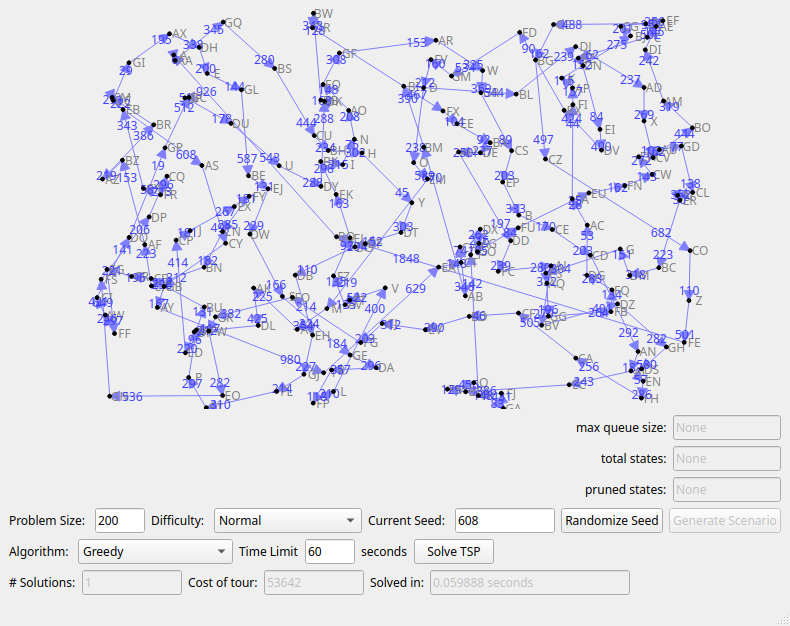
\includegraphics[scale=0.4]{greedy_example_200} \\
    \\
    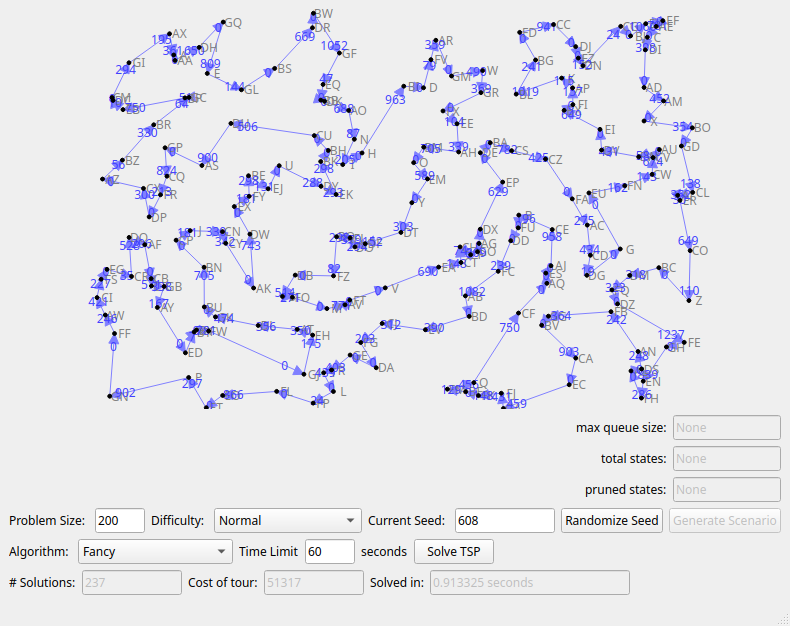
\includegraphics[scale=0.4]{fancy_example_200} \\

\begin{multicols}{2}
    From the pictures, you can clearly see the geometric effect that 2-opt has on the graph. As you see, it removes any edges that cross over each other, which generates a shorter overall path.
\end{multicols}

    \section{Results}
    \begin{adjustwidth}{-3cm}{100cm}
    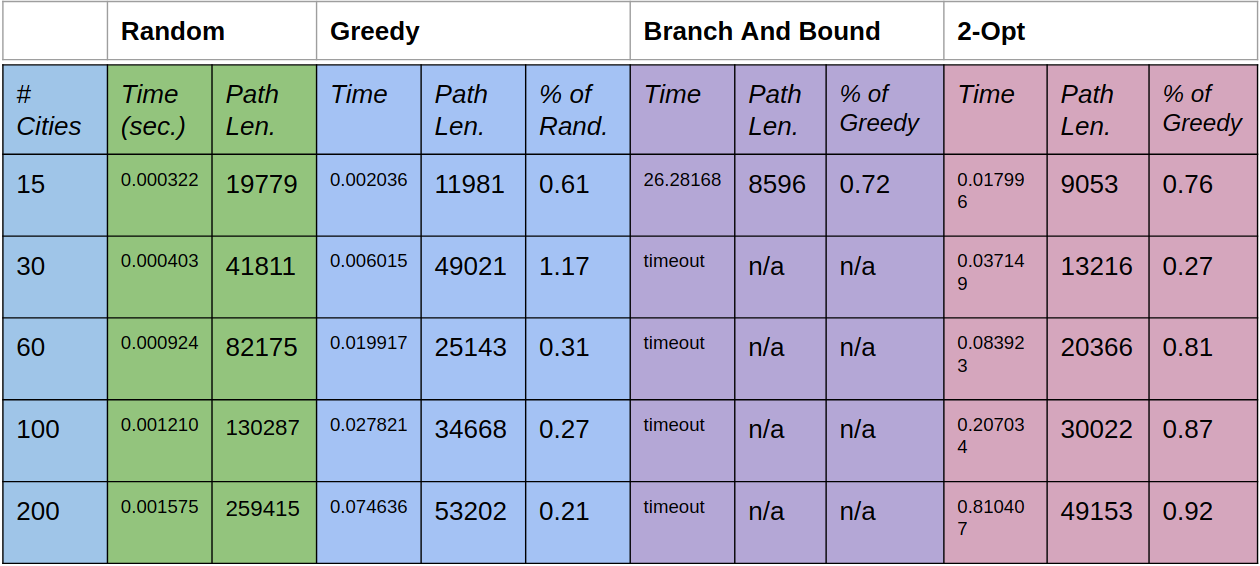
\includegraphics[scale=0.45]{table}
    \end{adjustwidth}

\begin{multicols}{2}
    \subsection{Analysis Of Results}
    One thing we learn from the data is that there is real difference. Considering how fast 2-opt runs, it is impressive that there were noticeable improvements. From this we can learn that deliberate effort can make a meaningful impact. From further testing, we discover that the upper limit of practicality is around 4,000 cities where it takes more than 10 minutes. Considering how hard a problem TSP is and how it consistently improves over other approximations, these are very impressive results. We found that the sweet spot was around 3000 cities, where the 2-opt stopped improving on the greedy by any significant amount.

    \section{Future Work}
    For further attempts, there are some considerations. The main concern is escaping local minimums with 2-opt. From our testing, this would require a more sophisticated approach than Monte Carlo. One possible approach would be running 2-opt on multiple initial solutions that might not be immediately as desirable, but might have a lower final solution.

    Another direction would be to use an entirely different solver for initial solutions than greedy. There are many approximations to this problem, each with their respective pros and cons. Much additional testing could discover the best future course of action for either of these shortcomings.
\end{multicols}


\end{document}
